\chapter{Introdução}
\label{capitulo:introducao}

Na última década, a quantidade e a qualidade dos modelos computacionais vem crescendo em um ritmo acelerado, o advento de hardwares mais poderosos viabilizou a construção de modelos que antes eram inviáveis como as redes neurais artificiais profundas.
Modelos cada vez mais sofisticados e complexos foram desenvolvidos e finalmente utilizados em uma escala maior, como as redes neurais convolucionais e os modelos generativos, que hoje produzem imagens, vídeos, sons e textos que possuem utilidade para diversas aplicações.
O contínuo desenvolvimento destes modelos, que hoje são a base de diferentes produtos e modelos de negócios, depende fundamentalmente da disponibilidade de conjuntos de dados apropriados. Não atoa, como uma espécie de senso comum, a indústria se refere aos dados como o novo petróleo.

Da escassez de dados e a natureza improvável de alguns fenômenos, emergem fortes motivações para o desenvolvimento de técnicas e ferramentas que possam mitigar os efeitos da falta de insumo para que a esteira de produção científica e industrial continue avançando e se beneficiando das capacidades destes modelos mais sofisticados.

Neste contexto, a utilização de modelos generativos como as \textit{Generative Adversarial Networks} (GANs) e os modelos de difusão se mostraram alternativas promissoras, produzindo resultados impressionantes para aplicações em diferentes áreas como saúde, finanças, agricultura, segurança e sensoriamento remoto \cite{iglesiasSurveyGANsComputer2023}.

Em uma rápida expansão na área de pesquisa de modelos generativos, muitos trabalhos foram publicados demonstrando resultados positivos sobre a utilização de dados sintetizados na produção de modelos computacionais para diferentes tarefas \cite{iglesiasSurveyGANsComputer2023}.
Porém, a própria natureza da avaliação de modelos generativos é complexa\cite{figueiraSurveySyntheticData2022}, consequentemente, implicando na necessidade de uma avaliação mais rigorosa sobre modelos e técnicas computacionais desenvolvidas sobre os dados artificiais.

Para definir se a utilização de dados artificiais produzem bons modelos, diversos trabalhos na literatura investigaram a qualidade dos conjuntos de dados gerados e dos modelos treinados sobre esses dados, utilizando o arcabouço de avaliação de eficácia de aprendizado de máquina. Neste arcabouço, um modelo é treinado em um conjunto de dados real, e outro em um conjunto de dados sintéticos, ambos para a realização da mesma tarefa, se a performance dos modelos for igual, ou melhor, conclui-se que os dados sintéticos são úteis para produzir bons modelos para a tarefa em questão, assim como ilustrado no esquema da figura \ref{fig:arcabouco-simples}.

\begin{figure}[htbp]
	\centering
	\caption[Arcabouço de avaliação de eficácia de aprendizado de máquina]{Arcabouço de avaliação de eficácia de aprendizado de máquina: a partir de dados reais e sintéticos, dois modelos são treinados para a mesma tarefa, ao fim, suas performances são avaliadas em um conjunto de dados real para se obter conclusões sobre a performance dos modelos e a utilidade dos dados sintéticos. Exemplo aplicado a um problema de classificação de imagens. }
		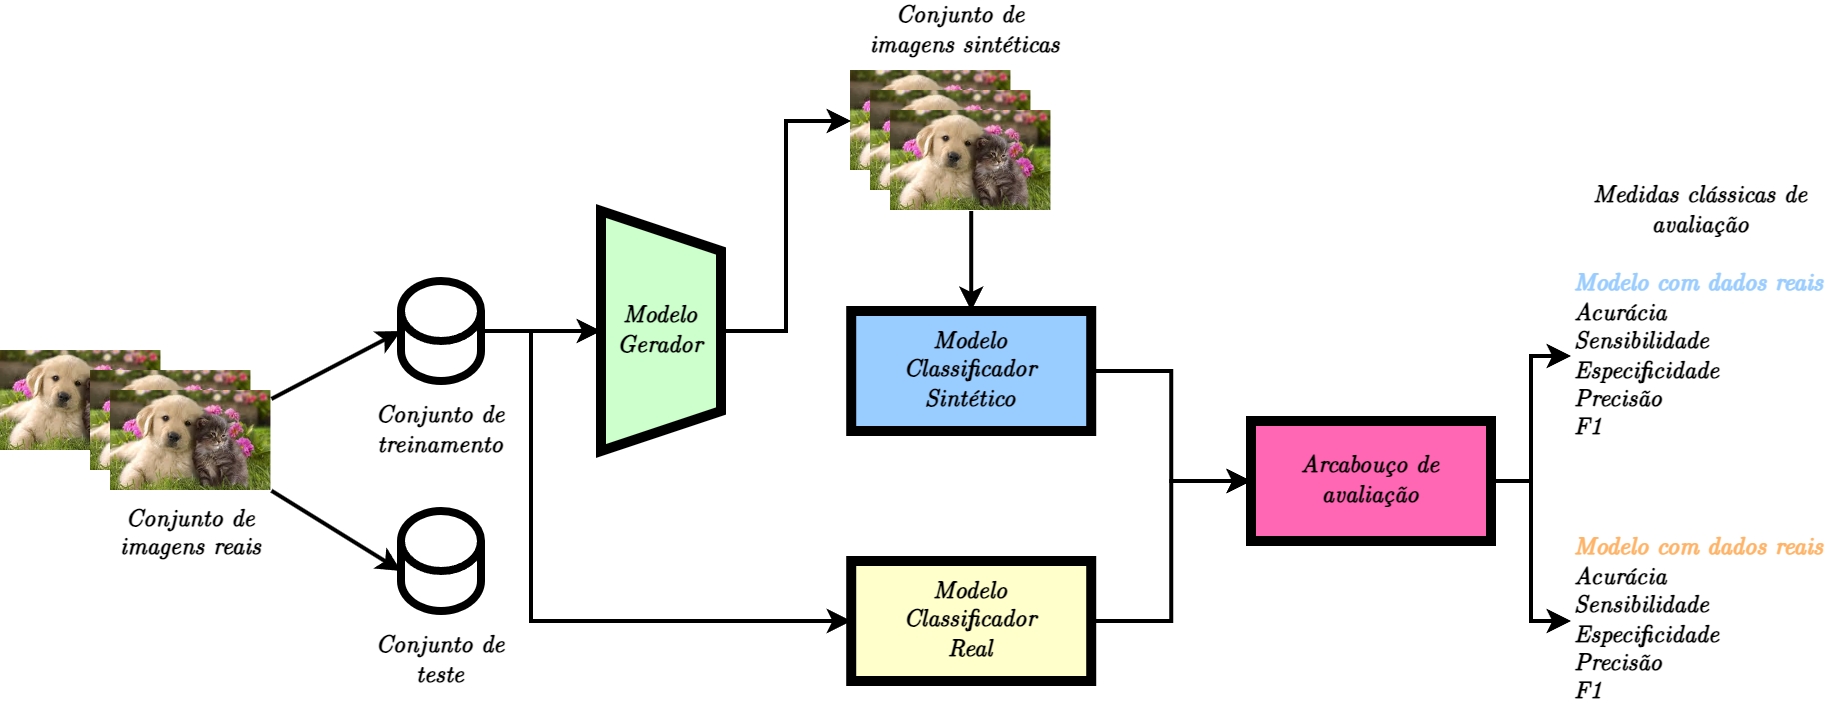
\includegraphics[scale=.25]{imagens/arcabouco-simples.png}
	\label{fig:arcabouco-simples}
  \source{Alexandre Farias, 2024}
\end{figure}

Apesar da utilização de métricas bem consolidadas, \citeonline{breimanStatisticalModeling2001} alerta que algumas classes de modelos computacionais podem sofrer do problema da multiplicidade de bons modelos, também conhecido como \textit{efeito Rashomon}. Neste caso, diferentes modelos de aprendizado de máquina podem resolver a mesma tarefa com performance similar em um conjunto de testes, mas por meio de relações e padrões diferentes encontrados nos dados de treinamento, a longo prazo, a utilização de cada dos modelos pode acarretar em diferentes erros de generalização ao observarem novas instâncias.

Neste contexto, é latente a necessidade da incorporação de métodos que permitam uma avaliação mais rigorosa de modelos construídos a partir de dados artificiais, métodos que nos permitam explicar suas previsões e assim entender com maior profundidade se a utilização de dados artificiais pode de fato suprir a escassez de dados, permitindo a continuidade dos avanços no desenvolvimento de modelos computacionais sob diferentes condições de disponibilidade de dados.

\section{Objetivo}

O objetivo deste trabalho é propor e desenvolver um arcabouço para avaliação do desempenho de modelos de \textit{deep learning} na tarefa de classificação de imagens, treinados em conjuntos de dados sintéticos e reais, levando em consideração métricas e conjuntos de dados padronizados, possibilitando que modelos treinados com conjuntos de dados reais e sintéticos - provenientes de diferentes modelos de geração de imagens - possam ser avaliados sob a luz de métricas que possibilitem a detecção de falhas de generalização e especificação.

Para este fim, técnicas de explicabilidade de modelos caixa-preta e processamento de imagens serão empregadas para o desenvolvimento de novas ferramentas que permitam avaliam com mais profundidade os modelos de classificação desenvolvidos.

\section{Hipótese}

Dado o contexto e objetivos supracitados, a hipótese do presente trabalho é de que a utilização de técnicas de explicabilidade e métodos clássicos de avaliação permitam avaliar com maior rigor se modelos de classificação treinados em dados sintetizados possuem a mesma performance e também aprendem relações semelhantes na tarefa de reconhecimento de padrões.

\section{Organização deste documento}

Para facilitar a leitura o presente trabalho está divido em capítulos, o capítulo \ref{capitulo:conceitos-fundamentais} explica os conceitos fundamentais que servem de base para o desenvolvimento deste trabalho, já o capítulo \ref{capitulo:revisao-bibliografica} discorre sobre trabalhos correlatos destacando seus métodos e resultados, por sua vez, o capítulo \ref{capitulo:estudo-piloto} apresenta resultados parciais já obtidos nesta pesquisa, por fim o capítulo \ref{capitulo:proposta} descreve em detalhes a proposta de pesquisa do presente trabalho.